% Chapter 1

\chapter{Implementation} % Main chapter title

\label{Chapter 5} % For referencing the chapter elsewhere, use \ref{Chapter1} 

\lhead{Chapter 5. \emph{Implementation}} % This is for the header on each page - perhaps a shortened title
We described in previous chapters of this thesis, the  problem  being addressed and our proposition for a solution. In the following, we present the implementation of this solution. 

\section{Development environment }
In order to implement the hybrid system Discolog, we used the collaborative discourse engine Disco \cite{rich2009building} as reactive HTN to which we integrate a Prolog STRIPS planner  to support the plan repair process. 

The most important challenge within the realization of such hybrid system is to support heterogeneous formalisms of Disco and STRIPS. The system must be able to convert  the HTN domain knowledge from procedural formalism implemented in Java to a declarative one capable to run in Prolog  and  handle exceptions related to this conversion. 

For that purpose, we integrated to Disco the tuProlog \footnote{\url{http://apice.unibo.it/xwiki/bin/view/Tuprolog/}}  java-based light-weight Prolog engine to create a bridge that can use the logical Prolog planner from the Java procedural environment . the environment architecture is described  in figure \ref{implementation environment of Discolog}.
\begin{figure}[h]
	\centering
	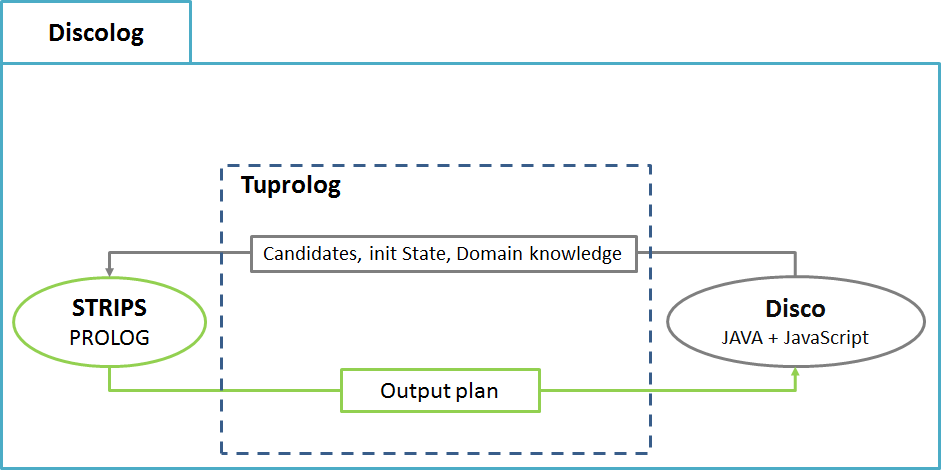
\includegraphics[width=\textwidth]{Pictures/archi1.png}
	\caption{\label{implementation environment of Discolog} implementation environment of Discolog}
\end{figure}


\section{Disco}
Disco \cite{rich2009building}is a collaborative discourse engine using reactive HTNS. The  most important feature of this reactive architecture is that allows the system to lead the user in a real time, without making any plan in advance. Disco's functional architecture is composed by a main component called \textit{task engine}. 
The function of the \textit{task engine}  is to load and validate a task model description and to maintain a representation of the current status of the user’s tasks.\cite{rich2009building}  


%----------------------------------------------------------------------------------------
\subsection{Disco task model}
Disco uses the ANSI/CEA-2018 standard for the procedural definition of the task model elements as described bellow :
\begin{itemize}
	\item \textit{Task}: The task model defines Task classes which are modeled using XML format, an example of the move\&paint implementation is showed in Appendix \ref{xml}. Primitive tasks may contain \textit{grounding script} parameter defined as JavaScript program which represent the effect of  the primitive task execution in the environment.
	
	\item \textit{Inputs and outputs} : Input includes all the data that may affect the execution of the task and output includes all data that can be affected by the execution of the task. these data type is defined in JavaScript.
	\item \textit{Conditions} : Task's conditions (Preconditions, postconditions ans applicability conditions) are defined as boolean JavaScript function to evaluate the execution of a task.

\end{itemize}

\section{Discolog implementation}
For the implementation of the Discolog system, we  faced some challenges. In addition to the management of heterogeneous environment, defining the level of information necessary to introduce in STRIPS domain knowledge required some reflection and designing a STRIPS planning algorithm able to provide effective solutions based on incomplete information in dynamic environment.
\subsection{The new Discolog API}
In order to implement the hybrid system Discolog we create an new  API divided in two mains folders :
	\begin{figure}[!h]
		\centering
		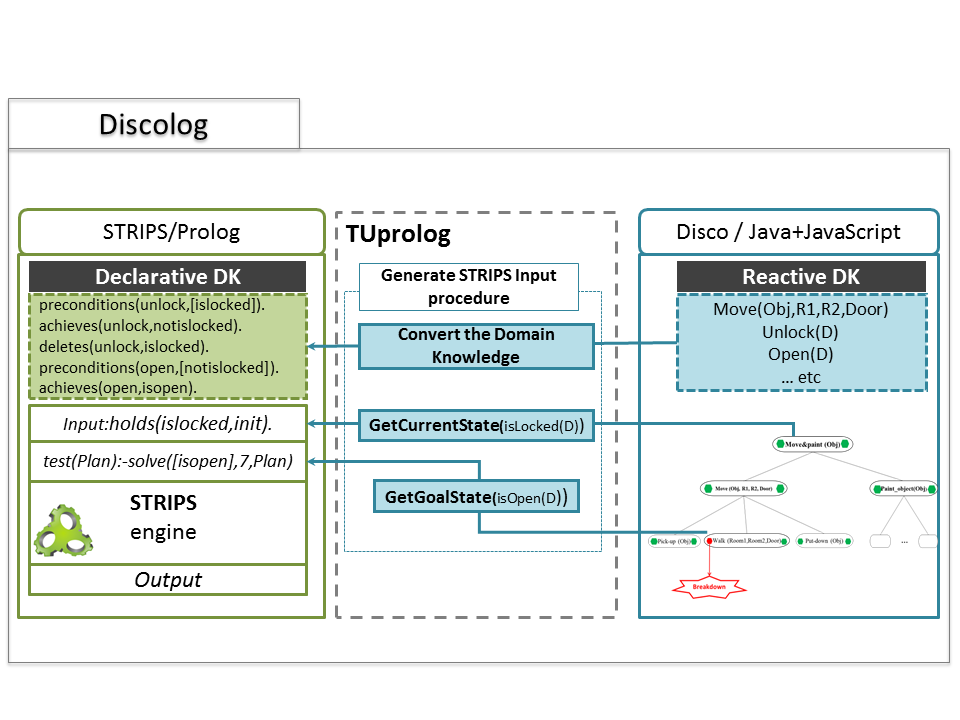
\includegraphics[width=\textwidth]{Pictures/input1.png}
		\caption{\label{input} Disco data generation in the moveandpaint example}
	\end{figure}
	
\subsubsection{ Disco extension }
We create an extension of Disco that can detect breakdowns and in such case, collects a candidates list for the plan recovery process. In addition, we manage to generate these candidates in the easiest way to be converted into Prolog formalism. The input Prolog planner is constituted in Disco via tuProlog as demonstrated in Figure \ref{input}.


 First, we start by creating the Prolog domain knowledge. Therefore, we extract all the primitives tasks and turn them to a Prolog formalism using tuProlog. Next, Disco observe the current state and convert it to the initial state. for example, in the move\&paint example, the current state where the breakdown occurs was IsLocked(Door) "the door is locked". Finally, the list of candidates is generated and each candidate is converted to a goal state to be achieve in Prolog.


\subsubsection{ Declarative Prolog implementation }
The main challenge faced in the creation of the STRIPS planner was to create an efficient means-end planning algorithm that can be integrated and executed  into tuProlog. Moreover, we had to define adequate structures that can receive the extracted domain knowledge. the STRIPS planner implemented is explained in Appendix \ref{AppendixB}.
% reference de STRIPS 


 Once STRIPS generate the plan recover, each action of this plan must be converted into primitive task formalism supported by Disco. Therefore we create a procedure that treat and convert the STRIPS plan output. An example of this procedure is shown  in Figure \ref{output} which describe how the plan repair is extracted for the move\&paint example. 

	\begin{figure}[!h]
		\centering
		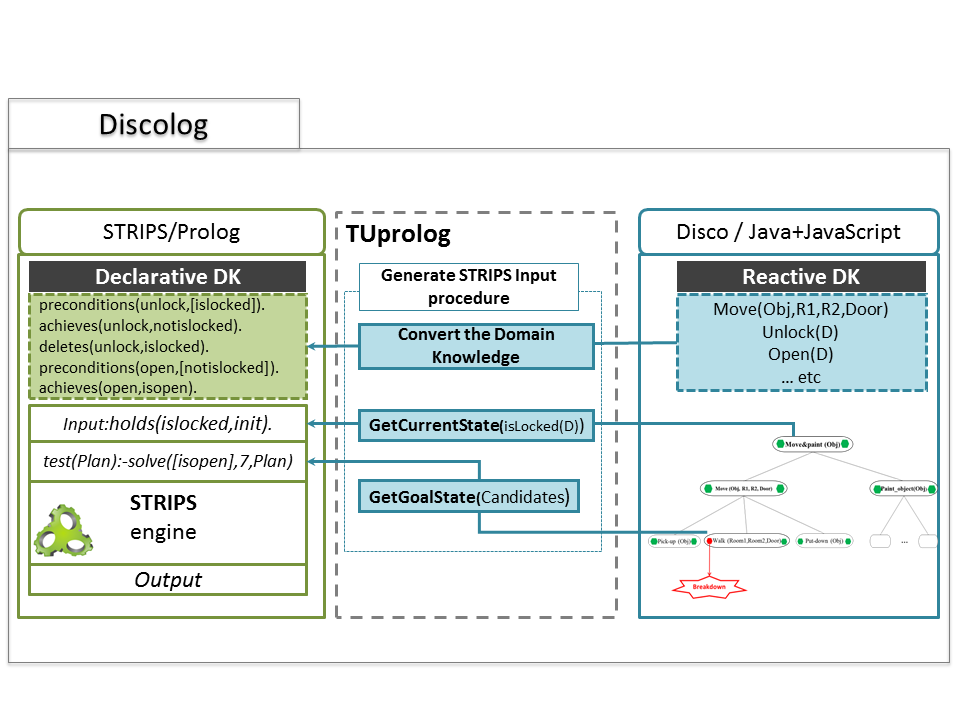
\includegraphics[width=\textwidth]{Pictures/output1.png}
		\caption{\label{output} Prolog data generation in the moveandpaint example}
	\end{figure}

\section{Conclusion}
In this chapter, we described the implementation of the Discolog system. First we introduce the environment of the implementation and we introduced the Disco system. Next we bring forward the new implemented Discolog API and explain each parts of this later.

In the next chapter, we present the experiments conducted to validate our system. 

%----------------------------------------------------------------------------------------


%\begin{multicols}{2}
%\lstinputlisting[language=XML]{Chapters/moveandpaint.xml}
%\end{multicols}
%\lstinputlisting[language=XML]{Chapters/moveandpaint.xml}
